\chapter{The CMS Detector}

The Compact Muon Solenoid (CMS) detector is a general-purpose detector for studying the physics of fundamental particles produced by proton-proton (\pp) and heavy ion collisions at the Large Hadron Collider (LHC) at CERN.
Two beams of protons circle the 27.6\unit{km} circumference of the LHC in opposite directions and collide at various locations along it; one of these locations is the CMS detector.

\section{The LHC}
The LHC is a circular hadron collider designed to collide protons at a center-of-mass energy of $\sqrt{s} = 14\TeV$ and at a design instantaneous luminosity of $\mathcal{L} = 10^{34} \cm^{-2} \unit{s}^{-1}$ \cite{Evans:2008zzb}.
Run 2 of the LHC began in 2015 with its superconducting dipole magnets operating such that the corresponding center-of-mass energy is $\sqrt{s} = 13\TeV$ \cite{Todesco:2017tcj}.

\section{The CMS Detector}
\subsection{Introduction}
\label{cms:intro}
CMS is located at Point~5 of the LHC in the commune of Cessy in eastern France.
It is named for two of its distinguishing features: its \textbf{m}uon system and its \textbf{s}olenoid magnet.
A large magnetic field with high bending power is required to precisely measure the momentum of high-energy charged particles.
This informs a choice of superconducting technology, and so a superconducting solenoid magnet sits at the heart of the cylindrically symmetric CMS detector, producing a continuous magnetic field of 4\unit{T}.
Muons are one of the five general categories of particles directly detected by CMS, and unique among them in that they neither stop nor decay within the boundaries of the detector.
They are less subject to energy losses when passing through detector material than electrons and so provide a powerful lens with which to study high-energy processes in the presence of high background.
The outermost bulk of CMS is thus a dedicated system for identifying and measuring muons, consisting of three kinds of gas ionization detectors \cite{Chatrchyan:2008zzk}.

The detector is structured like an onion, in layers, consisting of the following basic subsystems, ordered from innermost to outermost:
\begin{itemize}
  \item silicon tracker
  \item electromagnetic calorimeter
  \item hadronic calorimeter
  \item superconducting solenoid magnet
  \item muon system
\end{itemize}
\Fig~\ref{cms:interactive} is a diagram of a slice of the CMS detector illustrating these layers.
\begin{figure}[tpb]
  \centering
  \includegraphics[width=\textwidth]{figures/CMSSlice.png}
  \caption{Transverse slice of the CMS detector \cite{Davis:2205172}, illustrating the basic structure of CMS and the shapes of the tracks and energy deposits formed by the five general categories of particles directly detected by CMS by one or more of its subsystems.}
  \label{cms:interactive}
\end{figure}
It also shows the detector signatures of the general categories of particles directly detected by CMS:
\begin{itemize}
  \item electrons
  \item photons
  \item charged hadrons
  \item neutral hadrons
  \item muons
\end{itemize}
The charged particles -- electrons, muons, and charged hadrons -- are detected as they form curved, helical tracks in the silicon tracker (and in the case of muons, in the muon system as well).
Electrons, charged hadrons, and the neutral particles -- photons and neutral hadrons -- leave energy deposits in the electromagnetic and hadronic calorimeters.

\subsection{Coordinate System}
The origin of the coordinate system used by CMS is the nominal \pp collision point.
The $y$-axis points upwards, the $x$-axis points radially inwards towards the center of the LHC, approximately south, and thus the $z$-axis points approximately west.
The azimuthal angle $\phi$ is measured from the $x$-axis and the radial coordinate in the $xy$-plane is denoted $r$.
The polar angle measured from the $z$-axis is denoted $\theta$.
However, a more conventional coordinate used in hadron collider physics is the pseudorapidity $\eta$, defined as
\begin{equation}
  \eta = -\ln\tan\left(\frac{\theta}{2}\right)
  \label{eq:eta}
\end{equation}
For a particle of three-momentum $\vc{p}$ with $z$-component $p_z$, pseudorapidity can be written
\begin{equation}
  \eta = \frac12\ln\left(\frac{|\vc{p}|+p_z}{|\vc{p}|-p_z}\right)
  \label{eq:eta_p}
\end{equation}
This form elucidates its relationship to rapidity,
\begin{equation}
  y = \frac12\ln\left(\frac{E+p_z}{E-p_z}\right),
  \label{eq:rap}
\end{equation}
which is a quantity Lorentz invariant under boosts in the $z$-direction \cite{Hama:1981}.
The pseudorapidity has the advantage that it converges to rapidity in the high-velocity, low-mass limit (as $|\vc{p}|\to E$), but is only dependent on the polar angle $\theta$ and not on the energy of the particle.
\Fig~\ref{cms:quadrant} is a schematic diagram of one quadrant of CMS, showing the placement of the components of CMS within the coordinate system.
\begin{figure}[tpb]
  \centering
  \includegraphics[width=\textwidth]{figures/CMSGeometry.pdf}
  \caption{Schematic diagram of one quadrant of CMS in $r$-$z$ \cite{Sirunyan:2018fpa}, illustrating the position of all the subsystems with respect to the coordinate system, in both the barrel and the endcap.}
  \label{cms:quadrant}
\end{figure}

The diagram illustrates that $\eta = 0$ points upwards, while $\eta \to \infty$ points along the $z$-axis.
For this reason the ``forward'' regions close to the beamline (which are also less instrumented) are referred to as ``high $\eta$.''
The diagram also illustrates two distinct loci within the CMS detector: the barrel, which covers approximately (depending on subsystem) the region $|\eta| < 1.2$, and the endcap, which covers approximately (depending on subsystem) the region $1.2 < |\eta| < 3$.

\subsection{Silicon Tracker}
The inner tracking system of CMS must provide precise measurements of charged particle trajectories and reconstructions of secondary vertices of (on average) a thousand particles every 25\unit{ns} bunch crossing, exposed to the full flux of the radiation of the LHC.
These requirements on precision, speed, and radiation hardness inform a choice of silicon detector technology.
The ionization produced by an energetic charged particle passing through induces produced electron-hole pairs, which are measured as current in the presence of an applied voltage.

The CMS tracker consists of two silicon detector technologies: pixels and strips.
The innermost component of the tracker, closest to the collision point, is the pixel detector, consisting of three barrel layers and two endcap disks on each side of the barrel.
The silicon pixel sensors are $n$-on-$n$ devices, measuring $100 \times 150 \mum^2$, giving a spatial resolution of 15--20\mum and a transverse momentum ($\pT$) resolution of 1\% for 100\GeV particles.
Just outside the pixel detector is the strip detector, consisting of ten barrel layers and twelve endcap disks on each side of the barrel.
The silicon strip sensors are $p$-on-$n$ type microstrip sensors, manufactured on 6\unit{in} wafers \cite{Chatrchyan:2008zzk, CERN-LHCC-98-006, HARTMANN201225}.


\subsection{Electromagnetic Calorimeter}
The electromagnetic calorimeter (ECAL) was designed to achieve the excellent energy resolution critical for observing the decay of the SM Higgs to two photons: $H \to \gamma\gamma$.
The ECAL is a homogeneous calorimeter consisting of lead tungstate (PbWO$_4$) crystals, a material chosen for its high density and short radiation length.
Scintillation is the operating principle of the ECAL.
Electrons or photons passing through the detector material result in a cascade of electromagnetic interactions, producing a shower of particles culminating in a release of energy proportional to the energy of the incident particle.
The corresponding photons are then measured by photodetectors installed on each crystal \cite{Chatrchyan:2008zzk, CERN-LHCC-97-033, Fabjan:692252}.

\subsection{Hadronic Calorimeter}
The hadronic calorimeter (HCAL) is a sampling calorimeter, meaning it consists of repeating, alternating layers of an absorber, which degrades the energy of an incident particle, and an active medium, which provides a detectable signal.
This is in contrast to a homogenous calorimeter, like the ECAL, in which a single type of material performs both functions.

The HCAL consists of four parts: the barrel and endcap HCAL (HB and HE), the outer HCAL (HO), and the forward HCAL (HF).
In the HB and HE, the absorber material consists of thick tiles of brass, and the active medium consists of thinner tiles of scintillating plastic with wavelength-shifting readout fibers.
Brass is a dense material with many nuclei to interact strongly with incident hadron showers.
It is also non-magnetic, a necessary property of the absorber for the HB and HE which lie within the solenoid and experience its full 4\unit{T} magnetic field.

As the HB and HE lie within the solenoid and hence are only about 6 interaction lengths thick, the first layer of the muon system is instrumented with scintillator tiles, treating the solenoid as an additional absorber.
This ``tail catcher'' is known as the outer calorimeter, or HO.

The HF is located 11\unit{m} from the interaction point, in the pseudorapidity range of approximately $3.0 < |\eta| < 5.0$.
This forward region experiences very high levels of LHC radiation and thus is constructed out of radiation-hard materials: steel for the absorber and quartz fiber for the active material, which detects the Cerenkov radiation produced by energetic jets \cite{Chatrchyan:2008zzk, CERN-LHCC-97-031, Penzo2009}.

\subsection{Muon System}
As mentioned in \Sec~\ref{cms:intro}, muon detection is a powerful tool for studying high-energy processes in the presence of high background.
Because of the amount of material in the inner subsystems, typically only muons travel past the solenoid.
A track in the muon system therefore is associated with a muon.
Hadronic ``punchthrough'' in the muon system is minimal.

The muon system has three tasks: muon identification, muon reconstruction, and triggering.
As with the other subsystems, the shape of the solenoid informs a design of a cylindrical barrel section and an endcap disk section.
Both sections consist of four stations of muon detectors, concentric for the barrel and sequential for the endcap.
The muon system consists of three kinds of gaseous ionization detectors: drift tubes (DT), cathode strip chambers (CSC), and resistive plate chambers (RPC) \cite{Chatrchyan:2008zzk, CMS:1997dma}.

\subsubsection{Drift Tubes}
The barrel region of the muon system consists of four stations.
Drift tubes were chosen to be the tracking detectors in the barrel region in light of the low expected rate and relatively low intensity of the local magnetic field.
\Fig~\ref{cms:dt} is a diagram showing the principle of operation of a drift tube cell.
A cathode tube with cross-sectional dimensions $42 \times 13 \mm^2$ contains an anode wire (operating at 3600\unit{V}) under tension.
The tube is filled with a gas mixture of 85\% Ar and 15\% CO$_2$.
An energetic muon passing through this cell ionizes the gas, and the resulting electrons drift towards the wire.
Measuring the drift time (a maximum of 380\unit{ns}) yields a measurement of position within the cell.

The smallest independent unit of a DT is a superlayer (SL), consisting of four layers of drift cells staggered by a half cell.
A drift tube chamber consists of three (or two) SLs.
The wires in the two outer SLs are parallel to the beamline, and provide a track measurement in the $r$-$\phi$ (bending) plane.
The wires in the inner SL are orthogonal to the beamline, and measure the $z$-position along the beam.
This inner SL is not present in the fourth muon station, which consequently only measures the $\phi$ coordinate.

\begin{figure}[tpb]
  \centering
  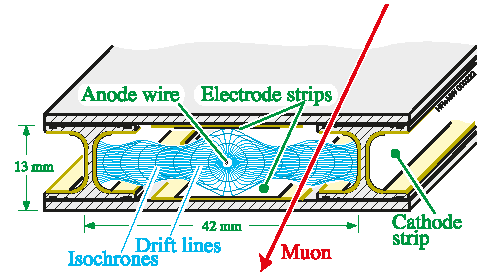
\includegraphics[width=0.8\textwidth]{figures/DT.pdf}
  \caption{Principle of operation of a drift tube cell \cite{Chatrchyan:2013sba}, showing the structure of a cell, as well as the drift lines and isochrones.}
  \label{cms:dt}
\end{figure}

\subsubsection{Cathode Strip Chambers}
The endcap region of the muon system consists of four stations.
Cathode strip chambers were chosen to be the tracking detectors in the endcap region for their excellent position resolution in the $\phi$ direction achieved by precision cathode charge readout and interpolation.
The CSCs are arranged in circular disks.
Each CSC consists of six layers, each layer lying in an $r$-$\phi$ plane of CMS, consisting of a gas mixture of 50\% CO$_2$, 40\% Ar, and 10\% CF$_4$ in between a plane of copper cathode strips and a plane of anode wires, operating at 2900--3600\unit{V}.
An energetic muon passing through a CSC ionizes the gas, and the resulting electrons drift towards the wires, causing an avalanche of charge that induces an opposite charge on the cathode strips.
Interpolating these charges yields a precise localization of the avalanche.
A more detailed overview of CSCs in the context of a study of neutron-induced background is given in \Sec~\ref{sec:csc_electronics}.

\subsubsection{Resistive Plate Chambers}
Interspersed throughout both the barrel and endcap muon system are resistive plate chambers, whose purpose is a fast time response and resolution comparable to that of scintillators.
RPCs therefore constitute a dedicated muon trigger for identifying muon tracks and assigning the bunch crossing with high efficiency.
An RPC consists of two parallel plates of phenolic resin coated with conductive graphite, with a 2\mm gap filled with a gas mixture of 95.2\% freon (C$_2$H$_2$F$_4$, known as R134a), 3.5\% isobutane (i-C$_4$H$_{10}$), and 0.3\% sulfur hexafluoride (SF$_6$).
An energetic muon crossing the chamber ionizes the gas and induces an image charge, which is sampled and read out.
The RPCs have a time resolution of about 2\unit{ns}, a much shorter time than the 25\unit{ns} between LHC bunch crossings, but much coarser position resolution than DTs or CSCs.

\subsection{Trigger System}
The LHC provides \pp collisions every 25\unit{ns}, corresponding to a crossing frequency of 40\unit{MHz}.
It is impossible to process and store this large amount of data synchronously with such a high rate, and so a rate reduction must be achieved, selecting a subset of the most interesting candidate events for physics analysis.
This rate reduction is performed by the CMS trigger system, an elaborate system of hardware and software that analyzes every bunch crossing and ``triggers'' on potentially interesting events.
The CMS trigger system operates in two steps.
The Level-1 (L1) trigger makes its decisions at the hardware level with custom-built programmable electronics, synchronously with the LHC.
The High-Level Trigger (HLT) makes its decisions at the software level, performing its computations offline with respect to the full rate of the LHC, more slowly than the L1 trigger, but faster than the full event readout.
The L1 trigger is designed to reduce the rate from 40\unit{MHz} to 100\unit{kHz}, and the HLT is designed to reduce the rate from 100\unit{kHz} to 100\unit{Hz} \cite{Chatrchyan:2008zzk, Adam:2005zf}.

The L1 trigger consists of a muon trigger and a calorimeter trigger, organized into local, regional, and global components.
Both the ECAL and all components of the HCAL participate in the calorimeter trigger, and all three muon chambers -- DTs, CSCs, and RPCs -- participate in the muon trigger, of which the RPCs are of particular importance to triggering due to their excellent time resolution.
The local components are the lowest level, based on energy deposits in the calorimeters and hits and segments in the muon system.
Regional components combine the information from the local components using pattern recognition and track finding and rank trigger objects in small regions.
The global components determine the highest-rank objects and transfer them to the global trigger of the L1 system.
The global trigger then makes the decision to reject or accept the event at Level-1.
A Level-1 Accept (L1A) decision is communicated to the subsystems and the event is passed to the HLT for further evaluation.
The L1 trigger must analyze every bunch crossing, doing so with a maximum latency of 3.2\mus.
\Fig~\ref{cms:L1} depicts the architecture of the L1 trigger.

\begin{figure}[tpb]
  \centering
  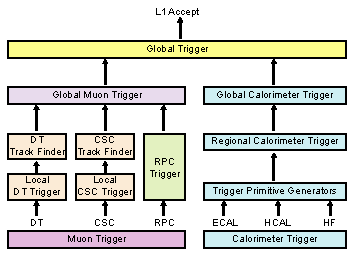
\includegraphics[width=0.8\textwidth]{figures/L1Architecture.pdf}
  \caption{Architecture of the L1 trigger system, based on a figure from \cite{Chatrchyan:2008zzk}, depicting the local, regional, and global components of the muon and calorimeter triggers, the information from which is processed by the global L1 trigger for trigger decision at L1.}
  \label{cms:L1}
\end{figure}

The L1 and HLT menus consists of paths that define criteria on which to trigger.
These criteria are the first step to any physics analysis, and so can include requirements on \pT, on numbers of muons or jets, on the geometry and angles between them, and much more.
The HLT uses information from the entire detector, with high-level algorithms that make a more precise decision than the coarser L1 trigger.
Each HLT path is seeded by one or more L1 paths and is designed to be inclusive and general while keeping the event rate as low as possible.
